%%%%%%%%%%%%%%%%%%%%%%%%%%%%%%%%%%%%%%%%%%%
%
% From a template maintained at https://github.com/jamesrobertlloyd/cbl-tikz-poster
%
% Code near the top should be fairly standard and not need to be changed
%  - except for the document class
% Code lower down is more likely to be customised
%
%%%%%%%%%%%%%%%%%%%%%%%%%%%%%%%%%%%%%%%%%%%


\documentclass[landscape,a0b,final,a4resizeable]{include/a0poster}


\usepackage{multicol}
\usepackage{color}
\usepackage{morefloats}
\usepackage[pdftex]{graphicx}
\usepackage{rotating}
\usepackage{amsmath, amsthm, amssymb, bm}
\usepackage{array}
\usepackage{booktabs}
\usepackage{multirow}
\usepackage{hyperref}


\usepackage{include/picins}
\usepackage{tikz}
\usetikzlibrary{shapes.geometric,arrows,chains,matrix,positioning,scopes,calc}
\tikzstyle{mybox} = [draw=white, rectangle]
\definecolor{darkblue}{rgb}{0,0.08,0.45}
\definecolor{blue}{rgb}{0,0,1}



\usepackage{nicefrac}
\newcommand{\vect}[1]{\underline{\smash{#1}}}
\renewcommand{\v}[1]{\vect{#1}}
\newcommand{\reals}{\mathds{R}}
\newcommand{\sX}{\mathcal{X}}
\newcommand{\sD}{\mathcal{D}}
\newcommand{\br}{}%{^{\text{\textnormal{ r}}}}
\newcommand{\cat}{^{\text{\textnormal{c}}}}

\usepackage{dsfont}

\ProvidesPackage{preamble}

\usepackage{url}
\usepackage{array}
\usepackage{amsmath,amssymb,amsfonts,textcomp,amsthm}
\usepackage{booktabs}
\usepackage{relsize}
\usepackage{nicefrac}
\usepackage{graphicx}
\usepackage{rotating}
\usepackage{nth}
\usepackage{acronym}
\usepackage{bm}
%\usepackage{caption} \DeclareCaptionType{copyrightbox}
\usepackage{footnote}
\usepackage{color}

\usepackage{tabularx}
\newcolumntype{x}[1]{>{\centering\arraybackslash\hspace{0pt}}m{#1}}
\newcommand{\tabbox}[1]{#1}

\usepackage{hyperref}
\definecolor{mydarkblue}{rgb}{0,0.08,0.45}
\hypersetup{
    pdftitle={},
    pdfauthor={},
    pdfsubject={},
    pdfkeywords={},
    pdfborder=0 0 0,
    pdfpagemode=UseNone,
    colorlinks=true,
    linkcolor=mydarkblue,
    citecolor=mydarkblue,
    filecolor=mydarkblue,
    urlcolor=mydarkblue,
    pdfview=FitH}

\newcommand{\asdf}{$^{\textnormal{th}}$}

\newcommand{\binarysum}{\sum_{\bf{x} \in \{0,1\}^D}}
\newcommand{\expect}{\mathbb{E}}
\newcommand{\expectargs}[2]{\mathbb{E}_{#1} \left[ {#2} \right]}
\newcommand{\var}{\mathbb{V}}
\newcommand{\varianceargs}[2]{\mathbb{V}_{#1} \left[ {#2} \right]}
\newcommand{\variance}{\mathbb{V}}
\newcommand{\cov}{\operatorname{cov}}
\newcommand{\Cov}{\operatorname{Cov}}
\newcommand{\covarianceargs}[2]{\Cov_{#1} \left[ {#2} \right]}
\newcommand{\colvec}[2]{\left[ \begin{array}{c} {#1} \\ {#2} \end{array} \right]}
\newcommand{\tbtmat}[4]{\left[ \begin{array}{cc} {#1} & {#2} \\ {#3} & {#4} \end{array} \right]}

%\newcommand{\covskinny}[2]{\var\!\left(#1\middle\vert#2\right)} 

\newcommand{\acro}[1]{\textsc{#1}}
%\newcommand{\vect}[1]{\boldsymbol{#1}}
\newcommand{\vect}[1]{{\bf{#1}}}
\newcommand{\mat}[1]{\mathbf{#1}}
\newcommand{\pderiv}[2]{\frac{\partial #1}{\partial #2}}
\newcommand{\npderiv}[2]{\nicefrac{\partial #1}{\partial #2}}

\newcommand{\pha}{^{\phantom{:}}}

\newcommand{\argmin}{\operatornamewithlimits{argmin}}
\newcommand{\argmax}{\operatornamewithlimits{argmax}}

% The following designed for probabilities with long arguments

\newcommand{\Prob}[2]{P\!\left(\,#1\;\middle\vert\;#2\,\right)}
\newcommand{\ProbF}[3]{P\!\left(\,#1\!=\!#2\;\middle\vert\;#3\,\right)}
\newcommand{\p}[2]{p\!\left(#1\middle\vert#2\right)}
\newcommand{\po}[1]{p\!\left(#1\right)}
\newcommand{\pF}[3]{p\!\left(\,#1\!=\!#2\;\middle\vert\;#3\,\right)} 
\newcommand{\mean}[2]{{m}\!\left(#1\middle\vert#2\right)}
%\newcommand{\novmean}[2]{{m}\!\left(#1\middle\vert#2\right)}
%\newcommand{\novcov}[2]{\var\!\left(#1\middle\vert#2\right)}
%\newcommand{\cov}[2]{\var\!\left(#1\middle\vert#2\right)} 
%\newcommand{\pskinny}[2]{p\!\left(#1\;\middle\vert\;#2\right)}
%\newcommand{\meanskinny}[2]{{m}\!\left(#1\middle\vert#2\right)}
%\newcommand{\covskinny}[2]{\var\!\left(#1\middle\vert#2\right)} 

\newcommand{\vI}{\mat{I}}
\newcommand{\vX}{\mat{X}}
\newcommand{\vY}{\mat{Y}}
\newcommand{\vZ}{\mat{Z}}
\newcommand{\vK}{\mat{K}}
\newcommand{\vs}{\vect{s}}
\newcommand{\va}{\vect{a}}
\newcommand{\vA}{\vect{A}}
\newcommand{\vb}{\vect{b}}
\newcommand{\vB}{\mat{B}}
\newcommand{\vR}{\mat{R}}
\newcommand{\vS}{\mat{S}}
\newcommand{\vu}{\vect{u}}
\newcommand{\vk}{\vect{k}}
\newcommand{\vc}{\vect{c}}
\newcommand{\vC}{\mat{C}}
\newcommand{\vw}{\vect{w}}
\newcommand{\vx}{\vect{x}}
\newcommand{\vy}{\vect{y}}
\newcommand{\vz}{\vect{z}}
\newcommand{\vmu}{\vect{\mu}}
\newcommand{\vpi}{\vect{\pi}}
\newcommand{\vphi}{\vect{\phi}}
\newcommand{\vSigma}{\mat{\Sigma}}
\newcommand{\vtheta}{\vect{\theta}}
\newcommand{\vl}{\vect{l}}
\newcommand{\vq}{\vect{q}}
\newcommand{\vf}{\vect{f}}
\newcommand{\vg}{\vect{g}}
\newcommand{\vell}{\vect{\ell}}
\newcommand{\ve}{\vect{\epsilon}}
\newcommand{\vzero}{\vect{0}}
\newcommand{\vone}{\vect{1}}

\newcommand{\He}{\mathcal{H}}
\newcommand{\normx}[2]{\left\|#1\right\|_{#2}}
\newcommand{\Hnorm}[1]{\normx{#1}{\He}}
\newcommand{\mmd}{{\rm MMD}}


\newcommand{\mf}{\bar{\vf}}

\newcommand{\st}{_\star}

\newcommand{\inv}{^{{\mathsmaller{-1}}}}
\newcommand{\tohalf}{^{{\mathsmaller{\nicefrac{1}{2}}}}}

\newcommand{\Normal}{\mathcal{N}}
\newcommand{\N}[3]{\mathcal{N}\!\left(#1|#2,#3\right)}
\newcommand{\Nt}[2]{\mathcal{N}\!\left(#1,#2\right)}
\newcommand{\bN}[3]{\mathcal{N}\big(#1|#2,#3\big)}
\newcommand{\boldN}[3]{\text{\textbf{\mathcal{N}}}\big(#1;#2,#3\big)}
\newcommand{\ones}[1]{\mat{1}_{#1}}
\newcommand{\eye}[1]{\mat{E}_{#1}}
\newcommand{\tra}{{^\ensuremath{\mathsf{T}}}}
\newcommand{\trace}{\operatorname{tr}}
\newcommand{\deq}{:=}
\newcommand{\degree}{^\circ}

\newcommand{\GPt}[2]{\mathcal{GP}\!\left(#1,#2\right)}

\DeclareMathOperator{\chol}{chol}
\DeclareMathOperator{\diag}{diag}

\newcommand{\gp}{{\acro{gp}}}
\newcommand{\gplvm}{{\acro{gp-lvm}}}
\newcommand{\bmc}{{\acro{bmc}}}
\newcommand{\bq}{{\acro{bq}}}
\newcommand{\sbq}{{\acro{sbq}}}

\newenvironment{narrow}[2]{%
  \begin{list}{}{%
  \setlength{\topsep}{0pt}%
  \setlength{\leftmargin}{#1}%
  \setlength{\rightmargin}{#2}%
  \setlength{\listparindent}{\parindent}%
  \setlength{\itemindent}{\parindent}%
  \setlength{\parsep}{\parskip}}%
\item[]}{\end{list}}



\newcommand{\dist}{\ \sim\ }
\def\given{\,|\,}

% Table stuff
\newcolumntype{C}[1]{>{\centering\let\newline\\\arraybackslash\hspace{0pt}}m{#1}}
\newcolumntype{L}[1]{>{\raggedright\let\newline\\\arraybackslash\hspace{0pt}}m{#1}}
\newcolumntype{R}[1]{>{\raggedleft\let\newline\\\arraybackslash\hspace{0pt}}m{#1}}


\def\ie{i.e.\ }
\def\eg{e.g.\ }
\def\iid{i.i.d.\ }
%\def\simiid{\sim_{\mbox{\tiny iid}}}
\def\simiid{\overset{\mbox{\tiny iid}}{\sim}}
\def\eqdist{\stackrel{\mbox{\tiny d}}{=}}
\newcommand{\distas}[1]{\mathbin{\overset{#1}{\kern\z@\sim}}}

\def\Reals{\mathbb{R}}

\def\Uniform{\mbox{\rm Uniform}}
\def\Bernoulli{\mbox{\rm Bernoulli}}
\def\GP{\mathcal{GP}}
\def\GPLVM{\mathcal{GP-LVM}}

% Kernel stuff

\def\inputVar{x}
\def\InputVar{X}
\def\InputSpace{\mathcal{X}}
\def\outputVar{y}
\def\OutputSpace{\mathcal{Y}}
\def\function{f}
\def\kernel{k}
\def\KernelMatrix{K}
\def\SumKernel{\sum}
\def\ProductKernel{\prod}
\def\expression{e}

\def\SE{\acro{SE}}
\def\Per{\acro{Per}}
\def\RQ{\acro{RQ}}
\def\Lin{\acro{Lin}}

\def\subexpr{{\cal S}}
\def\baseker{{\cal B}}
\def\numWinners{k}

\newcommand{\kSE}{{\acro{SE}}}
\newcommand{\kPer}{{\acro{Per}}}
\newcommand{\kLin}{{\acro{Lin}}}
\newcommand{\kRQ}{{\acro{RQ}}}


% Proof stuff
\theoremstyle{plain}
\newtheorem{theorem}{Theorem}[section]
\newtheorem{lemma}[theorem]{Lemma}
\newtheorem{prop}[theorem]{Proposition}
\newtheorem*{cor}{Corollary}

%\input{include/preamble2.sty}

%\usepackage{tabularx}

%%%%%%%%%%%%%%%%%%%%%%%%%%%%%%%%%%%%%%%%%%%
%
% myfig
%
% \myfig - replacement for \figure
% necessary, since in multicol-environment 
% \figure won't work        
%                 
%%%%%%%%%%%%%%%%%%%%%%%%%%%%%%%%%%%%%%%%%%%

\newcommand{\myfig}[3][0]{
\begin{center}
  \vspace{1.5cm}
  \includegraphics[width=#3\hsize,angle=#1]{#2}
  \nobreak\medskip
\end{center}}

%%%%%%%%%%%%%%%%%%%%%%%%%%%%%%%%%%%%%%%%%%%
%
% mycaption                
%
% \mycaption - replacement for \caption
% necessary, since in multicol-environment \figure and
% therefore \caption won't work
%
%%%%%%%%%%%%%%%%%%%%%%%%%%%%%%%%%%%%%%%%%%%

%\newcounter{figure}
\setcounter{figure}{1}
\newcommand{\mycaption}[1]{
  \vspace{0.5cm}
  \begin{quote}
    {{\sc Figure} \arabic{figure}: #1}
  \end{quote}
  \vspace{1cm}
  \stepcounter{figure}
}

%%%%%%%%%%%%%%%%%%%%%%%%%%%%%%%%%%%%%%%%%%%
%
% Some standard colours
%
%%%%%%%%%%%%%%%%%%%%%%%%%%%%%%%%%%%%%%%%%%%

\definecolor{camlightblue}{rgb}{0.601 , 0.8, 1}
\definecolor{camdarkblue}{rgb}{0, 0.203, 0.402}
\definecolor{camred}{rgb}{1, 0.203, 0}
\definecolor{camyellow}{rgb}{1, 0.8, 0}
\definecolor{lightblue}{rgb}{0, 0, 0.80}
\definecolor{white}{rgb}{1, 1, 1}
\definecolor{whiteblue}{rgb}{0.80, 0.80, 1}

%%%%%%%%%%%%%%%%%%%%%%%%%%%%%%%%%%%%%%%%%%%
%
% Some look and feel definitions
%
%%%%%%%%%%%%%%%%%%%%%%%%%%%%%%%%%%%%%%%%%%%

\setlength{\columnsep}{0.03\textwidth}
\setlength{\columnseprule}{0.0018\textwidth}
\setlength{\parindent}{0.0cm}

%%%%%%%%%%%%%%%%%%%%%%%%%%%%%%%%%%%%%%%%%%%
%
% \mysection - replacement for \section*
% 
% Puts a pretty box around some text
% TODO - any other thoughts for what this box should look like
%
%%%%%%%%%%%%%%%%%%%%%%%%%%%%%%%%%%%%%%%%%%%

\tikzstyle{mysection} = [rectangle, 
									draw=none, 
									shade, 
									outer color=camlightblue!30,
									inner color=camlightblue!30,
									text width=0.965\columnwidth,
									text centered,
									rounded corners=20pt,
									minimum height=0.09\columnwidth]

\newcommand{\mysection}[1]
{
\begin{center}
  \begin{tikzpicture}
    \node[mysection] {\sffamily\bfseries\LARGE#1};
  \end{tikzpicture}
\end{center}
}

%%%%%%%%%%%%%%%%%%%%%%%%%%%%%%%%%%%%%%%%%%%
%
% Set the font
%
% TODO - Not sure what a canonical choice is - feel free to modify
%
%%%%%%%%%%%%%%%%%%%%%%%%%%%%%%%%%%%%%%%%%%%

\renewcommand{\familydefault}{cmss}
\sffamily

%%%%%%%%%%%%%%%%%%%%%%%%%%%%%%%%%%%%%%%%%%%%%%%%%%%%
%%%               Background                     %%%
%%%%%%%%%%%%%%%%%%%%%%%%%%%%%%%%%%%%%%%%%%%%%%%%%%%%

\newcommand{\background}[3]{
  %\definecolor{cgradbegin}{#1}
  %\definecolor{cgradend}{#2}
 % \psframe[fillstyle=gradient,gradend=cgradend,
 % gradbegin=cgradbegin,gradmidpoint=#3](0.,0.)(1.\textwidth,-1.\textheight)
}




%%%%%%%%%%%%%%%%%%%%%%%%%%%%%%%%%%%%%%%%%%%%%%%%%%%%
%%%                pcolumn                       %%%
%%%%%%%%%%%%%%%%%%%%%%%%%%%%%%%%%%%%%%%%%%%%%%%%%%%%

\newenvironment{pcolumn}[1]{
  \begin{minipage}{#1\textwidth}
  \begin{center}
}{
  \end{center}
  \end{minipage}
}



%%%%%%%%%%%%%%%%%%%%%%%%%%%%%%%%%%%%%%%%%%%%%%%%%%%%
%%%                pbox                          %%%
%%%%%%%%%%%%%%%%%%%%%%%%%%%%%%%%%%%%%%%%%%%%%%%%%%%%

\definecolor{lcolor}{rgb}{0, 0, 0.80}
\definecolor{gcolor1}{rgb}{1, 1, 1}
\definecolor{gcolor2}{rgb}{.80, .80, 1}

  % \def\fc{fillcolor}
  % \def\getfc #1=#2\par{\def\ffc{#1} \ifx\ffc\fc #2\fi} 
  % \def\getfillcolor #1,#2\par{\getfc #1\par \getfc #2\par}

 %  \newcommand{\psshadowbox}[2]{%[2][magenta]{
%      \fbox{Input arg: #1}
%      \fbox{#1} 
%      \fbox {\getfillcolor #1\par}
%      \def\col{\getfillcolor #1\par}
 
%      \let\coll=\col
%       \coll
 %     \colorbox{\col}{#2}
%       \mbox
   %   \coloredshadowbox{black}{\coll}{#2}
%   }

\newcommand{\pbox}[4]{
%\psshadowbox[#3]{
%\fbox{
\mbox{
\begin{minipage}[t][#2][t]{#1}
#4
\end{minipage}
}%}
}

%%%%%%%%%%%%%%%%%%%%%%%%%%%%%%%%%%%%%%%%%%%
%
% Poster environment
%
% Centres everything and can be used to define the width of the content
%
%%%%%%%%%%%%%%%%%%%%%%%%%%%%%%%%%%%%%%%%%%%

\newenvironment{poster}{
  \begin{center}
  \begin{minipage}[c]{\textwidth}
}{
  \end{minipage}
  \end{center}
}

\def\newarrow{\mbox{\begin{tikzpicture}
             \useasboundingbox{(-3pt,-4.5pt) rectangle (19pt,1pt)};
             \draw[->] (0,-0.07)--(17pt,-0.07);\end{tikzpicture}}}




\newcommand\transpose{{\textrm{\tiny{\sf{T}}}}}
\newcommand{\note}[1]{}
\newcommand{\hlinespace}{~\vspace*{-0.15cm}~\\\hline\\\vspace*{0.15cm}}
\newcommand{\embeddingletter}{g}
\newcommand{\bo}{{\sc bo}}
%\newcommand{\gp}{{\sc gp}}
\newcommand{\agp}{Arc \gp}



\begin{document}
\begin{poster}

% Potentially add some space at the top of the poster
\vspace{0\baselineskip}



%%% Header
\begin{center}
\begin{pcolumn}{0.99}

\newcommand{\logowidth}{0.06\textwidth}  % width mauna decomp

\pbox{0.99\textwidth}{}{linewidth=2mm,framearc=0.3,linecolor=camdarkblue,fillstyle=gradient,gradangle=0,gradbegin=white,gradend=white,gradmidpoint=1.0,framesep=1em}{
%%% U Toronto Logo
\begin{minipage}[c]{\logowidth}
%  \begin{center}
    
\includegraphics[width=6.5cm,trim=9em 0em 9em 0em, clip]{badges/toronto}
 %       \vspace{.1in}
%    \includegraphics[width=6cm]{uot_text.gif}
%University of Cambridge 
%  \end{center}
\end{minipage}
%
%
%%% Cambridge Logo
\begin{minipage}[c]{\logowidth}
%  \begin{center}
    
\includegraphics[width=6cm]{badges/cambridgecrest}
    \vspace{.1in}
    
\includegraphics[width=6cm]{badges/unicamtext.pdf}
%University of Cambridge 
%  \end{center}
\end{minipage}
%
%
%%% Title
\begin{minipage}[c][9cm][c]{0.65\textwidth}
  \begin{center}
    {\sffamily \VeryHuge \textbf{Raiders of the Lost Architecture:\\Kernels for Bayesian Optimization \\in Conditional Parameter Spaces}}\\[10mm]
    {\huge\sffamily \Huge Kevin Swersky, David Duvenaud, Jasper Snoek, Frank Hutter, Michael Osborne\\[7.5mm]
    %\texttt{\{ti242, dkd23, zoubin\}@cam.ac.uk}
    }
  \end{center}
\end{minipage}
%
%
% Harvard
\begin{minipage}[c]{\logowidth}
  \begin{flushright}
%    
\includegraphics[width=6cm,angle=0]{badges/cambridgecrest}
%    \vspace{.1in}
%    
\includegraphics[width=6cm,angle=0]{unicamtext.pdf}
    
\includegraphics[width=8cm,trim=3.2em 0em 3.2em 2em, clip]{badges/harvard}
%University of Cambridge 
  \end{flushright}
\end{minipage}
%
\hspace{1cm}
% 
\begin{minipage}[c]{\logowidth}
%    
\includegraphics[width=6cm,angle=0]{badges/cambridgecrest}
%    \vspace{.1in}
%    
\includegraphics[width=6cm,angle=0]{unicamtext.pdf}
    
\includegraphics[width=8cm,trim=0em 0em 0em 0em, clip]{badges/freiburg}
\end{minipage}
%
\hspace{1cm}
% 
\begin{minipage}[c]{\logowidth}
%    
\includegraphics[width=6cm,angle=0]{badges/cambridgecrest}
%    \vspace{.1in}
%    
\includegraphics[width=6cm,angle=0]{unicamtext.pdf}
    
\includegraphics[width=8cm,trim=0em 0em 0em 0em, clip]{badges/oxford}
\end{minipage}

}
\end{pcolumn}
\end{center}

\vspace*{4cm}

\large


%%%%%%%%%%%%%%%%%%%%%%%%%%%%%%%%%%%%%%%%%%%%%%%%%%%%%%%%%%%%%%%%%%%%%%
%%% Begin of Document
%%%%%%%%%%%%%%%%%%%%%%%%%%%%%%%%%%%%%%%%%%%%%%%%%%%%%%%%%%%%%%%%%%%%%%


%%% Begin of Multicols-Enviroment
\begin{multicols}{3}
%%% Abstract
%\mysection{Summary}
%We introduce a Gaussian process model of functions which are $\textit additive$.  An additive function is one which decomposes into a sum of low-dimensional functions, each depending on only a subset of the input variables. 
%\begin{itemize}
%\item Most clustering methods assume a parametric form for each cluster, i.e. Gaussian.
%\item Our model is a Gaussian mixture that has been smoothly 'warped' to produce the observed clusters.
%\item Our model defines a non-parametric distribution over cluster shapes.
%\item Typically recovers a much smaller number of clusters, whose densities follow the contours of the data. 
%\item Can be viewed as a non-parametric manifold learning algorithm which doesn't require the construction of a nearest-neighbours graph.
%\end{itemize}
%\hspace{3cm}&
%\mysection{Motivation}
%\mysection{Sums of Kernels Correspond to Sums of GPs}
\mysection{The problem: Optimizing over architectures}
%

\vspace{0.5in}

\begin{minipage}[c]{0.17\textwidth}
\begin{itemize}
	\item Example: Optimizing hyperparameters of a neural net
	\item Deeper nets have more parameters.
	\item \textcolor{red} {Need to optimize over a varying number of parameters!}
\end{itemize}
\end{minipage}
\begin{minipage}[c]{0.15\textwidth}
\begin{centering}
\begin{tabular}{c}
\def\layersep{1.33cm}
\def\nodesep{.75cm}
\def\nodesize{.35cm}

\newcommand{\numdims}[0]{3}
\newcommand{\numhidden}[0]{4}
\newcommand{\upnodedist}[0]{0.6cm}
\newcommand{\bardist}[0]{\hspace{-0.2cm}}

\begin{tabular}{c|c}
\hspace{-0.5cm}
\begin{tikzpicture}[shorten >=1pt,->,draw=black!50, node distance=\layersep]
    \tikzstyle{every pin edge}=[<-,shorten <=1pt]
    \tikzstyle{neuron}=[circle,fill=black!25,minimum size=17pt,inner sep=0pt]
    \tikzstyle{input neuron}=[neuron, fill=green!50];
    \tikzstyle{output neuron}=[neuron, fill=red!50];
    \tikzstyle{hidden neuron}=[neuron, fill=blue!50];
    \tikzstyle{annot} = [text width=4em, text centered]

    % Draw the input layer nodes
    \foreach \name / \y in {1,...,\numdims}
    % This is the same as writing \foreach \name / \y in {1/1,2/2,3/3,4/4}
        \node[input neuron, minimum size=\nodesize
        %, pin=left:Input \#\y
        ] (I-\name) at (0,-\nodesep*\y) {};

    % Draw the hidden layer nodes
    \foreach \name / \y in {1,...,\numhidden}
        \path[yshift=0.5cm]
            node[hidden neuron, minimum size=\nodesize] (H-\name) at (\layersep,-\nodesep*\y) {};

    % Draw the output layer node
    \foreach \name / \y in {1,...,\numdims}
    	\node[output neuron, minimum size=\nodesize
    	%,pin={[pin edge={->}]right:Output }
    	] (O-\name) at (2*\layersep,-\nodesep*\y) {};

    % Connect every node in the input layer with every node in the
    % hidden layer.
    \foreach \source in {1,...,\numdims}
        \foreach \dest in {1,...,\numhidden}
            \path (I-\source) edge (H-\dest);

    % Connect every node in the hidden layer with the output layer
    \foreach \source in {1,...,\numhidden}
        \foreach \dest in {1,...,\numdims}
    	    \path (H-\source) edge (O-\dest);

    % Annotate the layers
%    \node[annot,above of=I-1, node distance=\upnodedist] {Inputs};
%    \node[annot,above of=H-1, node distance=\upnodedist] {Hidden};
%    \node[annot,above of=O-1, node distance=\upnodedist] {Outputs};
\end{tikzpicture}
&
\bardist
\begin{tikzpicture}[shorten >=1pt,->,draw=black!50, node distance=\layersep]
    \tikzstyle{every pin edge}=[<-,shorten <=1pt]
    \tikzstyle{neuron}=[circle,fill=black!25,minimum size=17pt,inner sep=0pt]
    \tikzstyle{input neuron}=[neuron, fill=green!50];
    \tikzstyle{output neuron}=[neuron, fill=red!50];
    \tikzstyle{hidden neuron}=[neuron, fill=blue!50];
    \tikzstyle{annot} = [text width=4em, text centered]

    % Draw the input layer nodes
    \foreach \name / \y in {1,...,\numdims}
    % This is the same as writing \foreach \name / \y in {1/1,2/2,3/3,4/4}
        \node[input neuron, minimum size=\nodesize
        %, pin=left:Input \#\y
        ] (I-\name) at (0,-\nodesep*\y) {};

    % Draw the hidden layer nodes
    \foreach \name / \y in {1,...,\numhidden}
        \path[yshift=0.5cm]
            node[hidden neuron, minimum size=\nodesize] (H-\name) at (\layersep,-\nodesep*\y) {};

    % Draw the hidden layer nodes
    \foreach \name / \y in {1,...,\numhidden}
        \path[yshift=0.5cm]
            node[hidden neuron, minimum size=\nodesize] (H2-\name) at (2*\layersep,-\nodesep*\y) {};


    % Draw the output layer node
    \foreach \name / \y in {1,...,\numdims}
    	\node[output neuron, minimum size=\nodesize
    	%,pin={[pin edge={->}]right:Output }
    	] (O-\name) at (3*\layersep,-\nodesep*\y) {};

    % Connect every node in the input layer with every node in the
    % hidden layer.
    \foreach \source in {1,...,\numdims}
        \foreach \dest in {1,...,\numhidden}
            \path (I-\source) edge (H-\dest);
            
    \foreach \source in {1,...,\numhidden}
        \foreach \dest in {1,...,\numhidden}
            \path (H-\source) edge (H2-\dest);            

    % Connect every node in the hidden layer with the output layer
    \foreach \source in {1,...,\numhidden}
        \foreach \dest in {1,...,\numdims}
    	    \path (H2-\source) edge (O-\dest);

    % Annotate the layers
%    \node[annot,above of=I-1, node distance=\upnodedist] {Inputs};
%    \node[annot,above of=H-1, node distance=\upnodedist] {Hidden};
%    \node[annot,above of=H2-1, node distance=\upnodedist] {Hidden};
%    \node[annot,above of=O-1, node distance=\upnodedist] {Outputs};
\end{tikzpicture}
\bardist
 \\
\hspace{-0.5cm} One-layer MLP & 
Two-layer MLP 
\end{tabular}
 \\
%\textcolor{darkblue}{ [Rasmussen, 1999]}
\end{tabular}
\end{centering}
\end{minipage}

\vspace{0.5in}

\mysection{Bayesian Optimization with Guassian Processes}
Formally, we aim to do inference about some function $f$ with domain 
%(input space)
 $\sX$. $\sX = \prod_{i=1}^D \sX_i$ is a $D$-dimensional input space, where each individual dimension is bounded real, that is, $\sX_i = [l_i, u_i] \subset \reals$ (with lower and upper bounds $l_i$ and $u_i$, respectively). We define functions $\delta_i\colon \sX\to \{\text{true}, \text{false}\}$, for $i \in \{1,\,\ldots,\,D\}$. $\delta_i(\v{x})$ stipulates the relevance of the $i$th feature $x_i$ to 
 %inference about
  $f(\v{x})$.



\subsection{The problem}
\vspace{-0.05in}

As an example, imagine trying to model the performance of a neural network having either one or two hidden layers, with respect to the regularization parameters for each layer, $x_1$ and $x_2$.  If $y$ represents the performance of a one layer-net with regularization parameters $x_1$ and $x_2$, then the value $x_2$ doesn't matter, since there is no second layer to the network. Below, we'll write an input triple as $(x_1, \delta_2(\v{x}), x_2)$ and assume that $\delta_1(\v{x}) = \text{true}$; that is, the regularization parameter for the first layer is always relevant. 

In this setting, we want a kernel $k$ to be dependent on which parameters are relevant, and the values of relevant parameters for both points. For example, consider first-layer parameters $x_1$ and $x_1'$:
%
\begin{itemize}
\item If we are comparing two points for which the same parameters are relevant, the value of any unused parameters shouldn't matter,  
\begin{equation}
 k\bigl((x_1, \textnormal{false}, x_2), (x_1', \textnormal{false}, x_2') \bigr)
= k\bigl((x_1, \textnormal{false}, x_2''), (x_1', \textnormal{false}, x_2''')\bigr),\ 
\forall x_2, x_2', x_2'', x_2''';
\end{equation}
\item The covariance between a point using both parameters and a point using only one should again only depend on their shared parameters,
\begin{equation}
 k\bigl((x_1, \textnormal{false}, x_2), (x_1', \textnormal{true}, x_2') \bigr)
= k\bigl((x_1, \textnormal{false}, x_2''), (x_1', \textnormal{true}, x_2''')\bigr),\ 
\forall x_2, x_2', x_2'', x_2'''.
\end{equation}
\end{itemize}




\newpage 
\mysection{The Arc Kernel}

We can build a kernel with these properties for each possibly irrelevant input dimension $i$ by embedding our points into a Euclidean space.  Specifically, the embedding we use is
%
%To emphasize that we're in the real case, we explicitly denote the pseudometric as $d\br_i$ and the (pseudo-)isometry from $(\sX, d_i)$ to $\reals^2,d_\text{E}$ 
%as $f\br_i$. For the definitions, recall that $\delta_i(\v{x})$ is true iff dimension $i$ is relevant given the instantiation of $i$'s ancestors in $\v{x}$.
%
%
\begin{equation}
\embeddingletter_i\br(\v{x}) = \left\{\begin{array}{ll}
[0,0]^\transpose & \textrm{ if } \delta_i(\v{x}) = \textrm{ false }\\
\omega_i [\sin{\pi\rho_i\frac{x_i}{u_i-l_i}}, \cos{\pi\rho_i\frac{x_i}{u_i-l_i}}]^\transpose & \textrm{ otherwise.}\end{array}\right.
\label{eq:embedding}
\end{equation}
Where $\omega_i \in \mathbb{R}^+$ and $\rho_i \in [0,1]$.
%
%\begin{figure}
%	\floatbox[{\capbeside\thisfloatsetup{capbesideposition={right,top}}}]{figure}[\FBwidth]

%\begin{table}
%\begin{tabular}{c}

\centering
% A simple figure to illustrate Mike and Frank's embedding
% Sept 2013

\newcommand{\scaleamount}{0.7}
\newcommand{\anglemin}{40}
\newcommand{\angleminplusone}{41}
\newcommand{\anglemax}{150}
\newcommand{\angleone}{70}
\newcommand{\angletwo}{120}
\newcommand{\bigradius}{3}
\newcommand{\biggerradius}{3.3}
\newcommand{\smallradius}{0.5}
\newcommand{\xtwolabelangle}{90}
\newcommand{\belowamount}{0.2cm}
\newcommand{\belowamounttwo}{0.11cm}
\newcommand{\myell}{l}
\newcommand{\embedding}{g}

%\begin{center}
%\framebox{
\begin{tikzpicture}
[trans/.style={thick,->,shorten >=2pt,shorten <=2pt,>=stealth},scale=\scaleamount, every node/.style={transform shape}]

\tikzset{state/.style={circle,draw=black, very thick,minimum size=4em}}

\def\centerarc[#1] (#2) (#3:#4:#5)% [draw options] (center) (initial angle:final angle:radius)
{ \draw[#1] (#2) ++(#3:#5) arc (#3:#4:#5);
}
	\coordinate (left) at ({\bigradius*cos(\anglemax)}, {\bigradius*sin(\anglemax)});
	\coordinate (right) at ({\bigradius*cos(\anglemin)}, {\bigradius*sin(\anglemin)});

	\coordinate (O1) at (-2, 0);
	\coordinate (O2) at (3, 1);
	
	\coordinate (left1) at ($ (left) + (O1) $);
	\coordinate (right1) at ($ (right) + (O1) $);
	\coordinate (left2) at ($ (left) + (O2) $);
	\coordinate (right2) at ($ (right) + (O2) $);
	
	% First arc
	% ==================
	
	% Draw arcs
	\centerarc[thick] (O1) (\anglemin:\anglemax:\bigradius)
	\centerarc[thick] (O1) (\anglemin:\anglemax:\smallradius)

	\draw[fill] (left1) circle (1.5pt);
	\draw (left1) node[below = \belowamount, right] {$\embedding(0, \textnormal{true}, u$)};
	
	\draw[fill] (right1) circle (1.5pt);
	\draw (right1) node[below = \belowamount] (r1below) {}
	               node[left] {$\embedding(0, \textnormal{true}, \myell)$};

	\draw[fill] (O1) circle (1.5pt);
	\draw (O1) node[below = \belowamount] (o1below) {}
	           node[left = 0.3cm] {$\embedding(0, \textnormal{false}, \cdot)$};

	\draw (left1) -- (O1) node[above] {$\rho \pi$};
	\draw (right1) -- (O1) node[midway, below] {$\omega$};
	
	
	% Second arc
	% ================================
	\centerarc[thick] (O2) (\anglemin:\anglemax:\bigradius)
	\centerarc[thick] (O2) (\anglemin:\anglemax:\smallradius)

	\draw[fill] (left2) circle (1.5pt);
	
	\draw[fill] (right2) circle (1.5pt);
	\draw (right2) node[below = \belowamount] (r2below) {};
	

	\draw[fill] (O2) circle (1.5pt);
	\draw (O2) node[below = \belowamount] (o2below) {}
                   node[right] {$\embedding(1, \textnormal{false}, \cdot)$};

	\draw[dashed] (left2) -- (O2);
	\draw[dashed] (right2) -- (O2);


	% Connect the arcs
	\draw (left1) -- (left2);
	\draw (right1) -- (right2);
	\draw[thick] (O1) -- (O2);
	
	% Draw surface
	\foreach \i in {\angleminplusone, ..., \anglemax}
	{
		\coordinate (arca) at ({\bigradius*cos(\i)}, {\bigradius*sin(\i)});
		\coordinate (arcb) at ({\bigradius*cos(\i - 1)}, {\bigradius*sin(\i - 1)});
		\coordinate (arca1) at ($ (arca) + (O1) $);
		\coordinate (arca2) at ($ (arca) + (O2) $);
		\coordinate (arcb1) at ($ (arcb) + (O1) $);
		\coordinate (arcb2) at ($ (arcb) + (O2) $);
%		\draw[green] (arca1) -- (arca2);
		\fill[fill=blue!40,fill opacity=0.8](arca1)--(arca2)--(arcb2)--(arcb1)--cycle;
	}

	\draw (right2) node[left] {$\embedding(1, \textnormal{true}, \myell)$};

	% Draw arrows showing in which direction x1 varies.
	\coordinate(x1half) at ($ (right1)!0.5!(right2) $);
	\draw (x1half) node[below = \belowamounttwo] (x1halfbelow) {$x_1$};
	\draw[trans] ($ (r1below)!0.45!(r2below) $) -- ($ (r1below)!0.3!(r2below) $);
	\draw[trans] ($ (r1below)!0.55!(r2below) $) -- ($ (r1below)!0.7!(r2below) $);

	\coordinate(x2half) at ($ (O1)!0.6!(O2) $);
	\draw (x2half) node[below = \belowamounttwo] (x2halfbelow) {$x_1$};
	\draw[trans] ($ (o1below)!0.55!(o2below) $) -- ($ (o1below)!0.4!(o2below) $);
	\draw[trans] ($ (o1below)!0.65!(o2below) $) -- ($ (o1below)!0.8!(o2below) $);

	% Draw arrows showing in which direction x2 varies.
	\coordinate (arclabel) at ($ (O1) + ({\biggerradius*cos(\xtwolabelangle)}, {\biggerradius*sin(\xtwolabelangle)}) $);
	\draw (arclabel) node {$x_2$};
	\centerarc[trans] (O1) ( \xtwolabelangle + 5  :  \xtwolabelangle + 30  :\biggerradius)
	\centerarc[trans] (O1) ( \xtwolabelangle - 5  :  \xtwolabelangle - 30  :\biggerradius)

%	\coordinate (x1) at ({\bigradius*cos(\angletwo)}, {\bigradius*sin(\angletwo)});
%	\coordinate (x2) at ({\bigradius*cos(\angleone)}, {\bigradius*sin(\angleone)});
%	\draw[fill] (x1) circle (1.5pt);
%	\draw (x1) node[above, left] {$f(x_1, \textnormal{true})$};
%	\draw[fill] (x2) circle (1.5pt);
%	\draw (x2) node[above, right] {$f(x_2, \textnormal{true})$};
\end{tikzpicture}
%}
%\end{center}
\label{fig:cylinder}
	%\caption{}
%  The parameter $\rho$ determines how much distance there is along the arc.
%\end{figure}
%\end{tabular}

A demonstration of the embedding giving rise to the pseudo-metric.  All points for which $\delta_2(x) =$ false are mapped onto a line varying only along $x_1$.  Points for which $\delta_2(x) =$ true are mapped to the surface of a semicylinder, depending on both $x_1$ and $x_2$.  This embedding gives a constant distance between pairs of points which have differing values of $\delta$ but the same values of $x_1$.
%\end{table}


Figure \ref{fig:cylinder} shows a visualization of the embedding of points $(x_1, \delta_2(\v{x}), x_2)$ into $\reals^3$. 
%
In this space, we have the Euclidean distance,
%
\begin{equation}
d\br_i(\v{x}, \v{x}') = ||\embeddingletter_i\br(\v{x})-\embeddingletter_i\br(\v{x}')||_2 =\left\{\begin{array}{ll}
0 & \textrm{ if } \delta_i(\v{x}) = \delta_i(\v{x}') = \textrm{false}\\
\omega_i & \textrm{ if } \delta_i(\v{x}) \neq \delta_i(\v{x}')\\
\omega_i \sqrt{2} \sqrt{1 - \cos(\pi\rho_i \frac{x_i-x_i'}{u_i-l_i})} & \textrm{ if } \delta_i(\v{x}) = \delta_i(\v{x}') = \textrm{true}. \end{array}\right.
\label{eq:distance}
\end{equation}







\newpage




\mysection{Regression Results}

\begin{minipage}[c]{0.95\columnwidth}
%\begin{table}[h!]
%\caption{{\small \label{tab:nn_error}}}
%\label{tbl:nn_nmse}
% --- Automatically generated by resultsToLatex4.m ---
% Exported at 20-Oct-2013 19:39:08
\begin{center}
\begin{tabular}{l | r r}
Method & \rotatebox{0}{ Original data   }  & \rotatebox{0}{ Log outputs }  \\ \hline
Separate Linear & $0.812 \pm 0.045$ & $0.737 \pm 0.049$ \\
Separate \gp{} & $0.546 \pm  0.038$ & $0.446 \pm 0.041$ \\
Separate \agp{} & $0.535 \pm 0.030$ & $0.440 \pm 0.031$ \\
Linear & $0.876 \pm 0.043$ & $0.834 \pm 0.047$ \\
\gp{} & $0.481 \pm 0.031$ & $0.401 \pm 0.028$ \\
\agp{} & $\mathbf{0.421 \pm  0.033}$ & $\mathbf{0.335 \pm 0.028}$
\end{tabular}
\end{center}
% End automatically generated LaTeX


Normalized Mean Squared Error on MNIST Bayesian optimization data
%% --- Automatically generated by resultsToLatex4.m ---
% Exported at 20-Oct-2013 19:39:08
\begin{center}
{\small
\begin{tabular}{l | r r r r r r}
Method & Separate Linear & Separate \gp{} & Separate \agp{} & Linear & \gp{} &\agp{} \\ \hline
Original data & $0.812 \pm 0.045$ & $0.546 \pm 0.038$ & $0.535 \pm 0.030$ & $0.876 \pm 0.043$ & $0.481 \pm 0.031$ & $\mathbf{0.421 \pm 0.033}$ \\
Log outputs   & $0.737 \pm 0.049$ & $0.446 \pm 0.041$ & $0.440 \pm 0.031$ & $0.834 \pm 0.047$ & $0.401 \pm 0.028$ & $\mathbf{0.335 \pm 0.028}$ \\
\end{tabular}
}
\end{center}
% End automatically generated LaTeX

%\caption{Regression errors for a GP with the arc kernel compared to baselines.}
%\end{table}
\end{minipage}




\mysection{Optimization Results}

%\begin{figure}[t!]
	\centering
%	\begin{subfigure}[]{0.3\textwidth}
\begin{tabular}{cc}
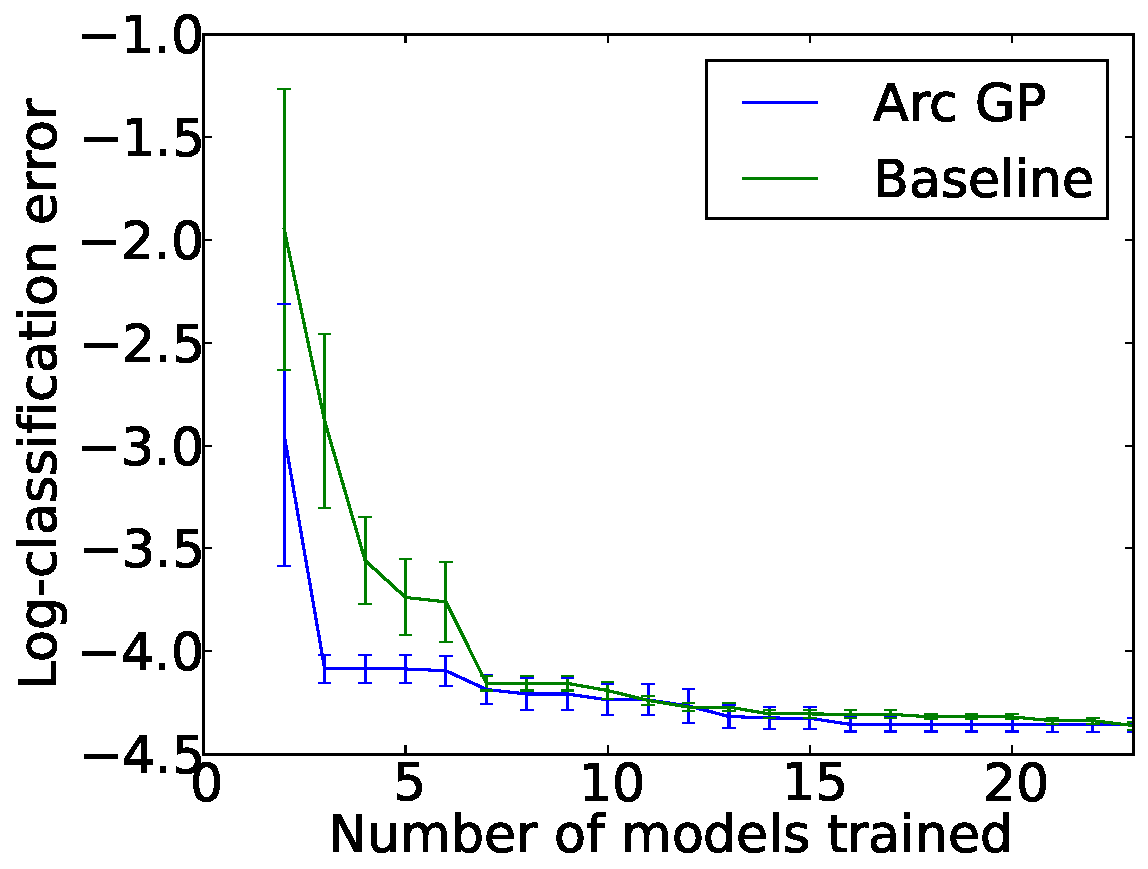
\includegraphics[width=0.45\columnwidth]{figures/mnist.pdf} &
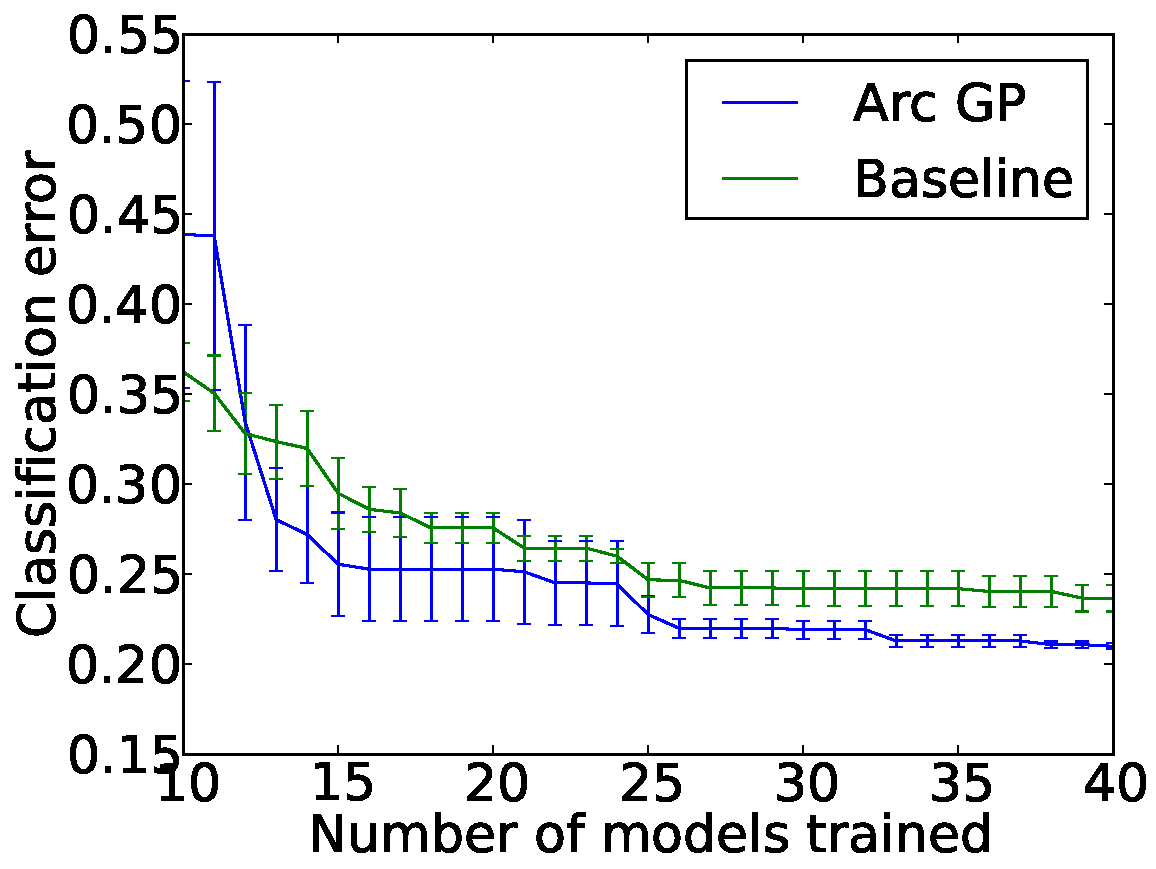
\includegraphics[width=0.45\columnwidth]{figures/cifar10.pdf} \\
MNIST &  CIFAR-10
\end{tabular}		


\begin{tabular}{c}
		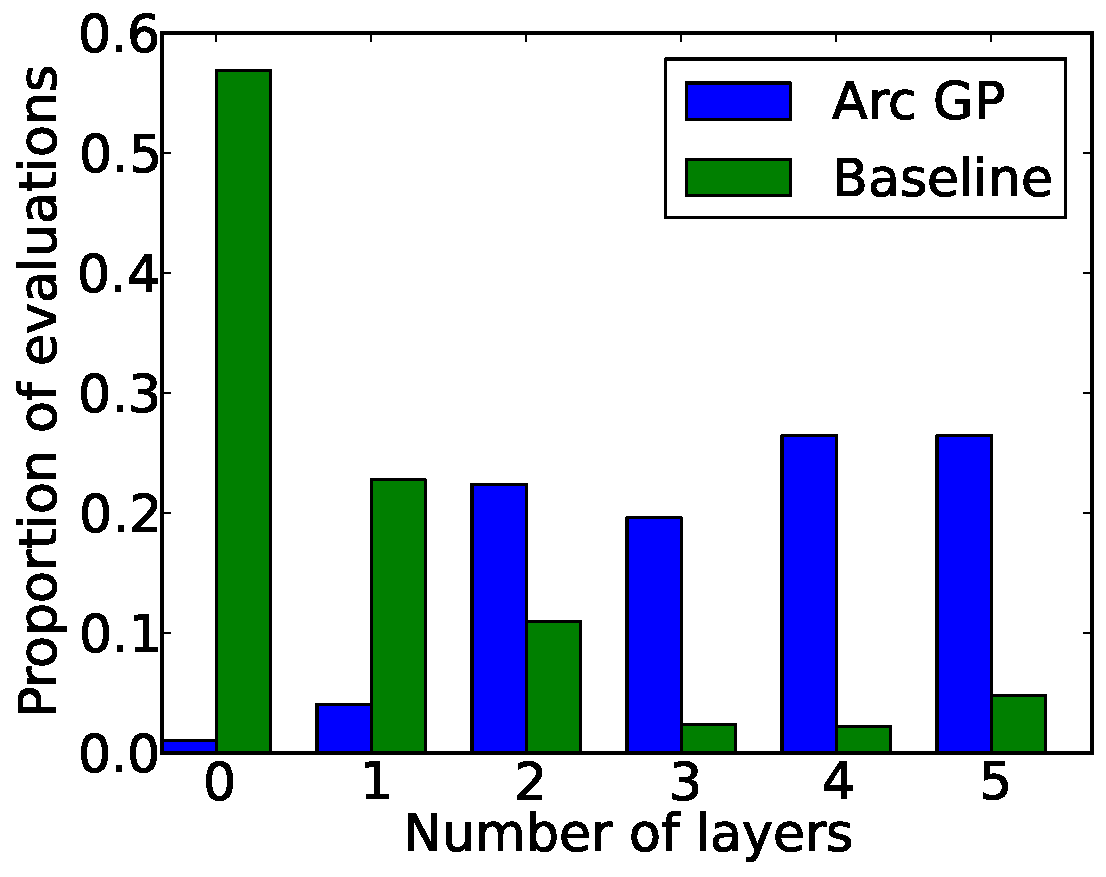
\includegraphics[width=0.45\columnwidth]{figures/fevals_per_layer.pdf} \\
Architectures searched
\end{tabular}
		
%		\label{fig:proparchs}
%	\end{subfigure}
%	\caption{Bayesian optimization results using the arc kernel.}
%	\label{fig:arcbo}
%\vspace{-0.3cm}
%\end{figure}


\mysection{Future Work}

	\begin{itemize}
		\item More experiments...
	\end{itemize}

%\paragraph{Code}
Code available at \texttt{http://???}

Paper available at \texttt{http://???}


%The related HKL framework

%\subsubsection*{Acknowledgments}
%The authors would like to thank John Chew and Guillaume Obozonksi for their helpful comments.

%\end{thebibliography}

\end{multicols}
\end{poster}
\end{document}

